\chapter{Retrospective Spring}

\begin{figure}[!ht]
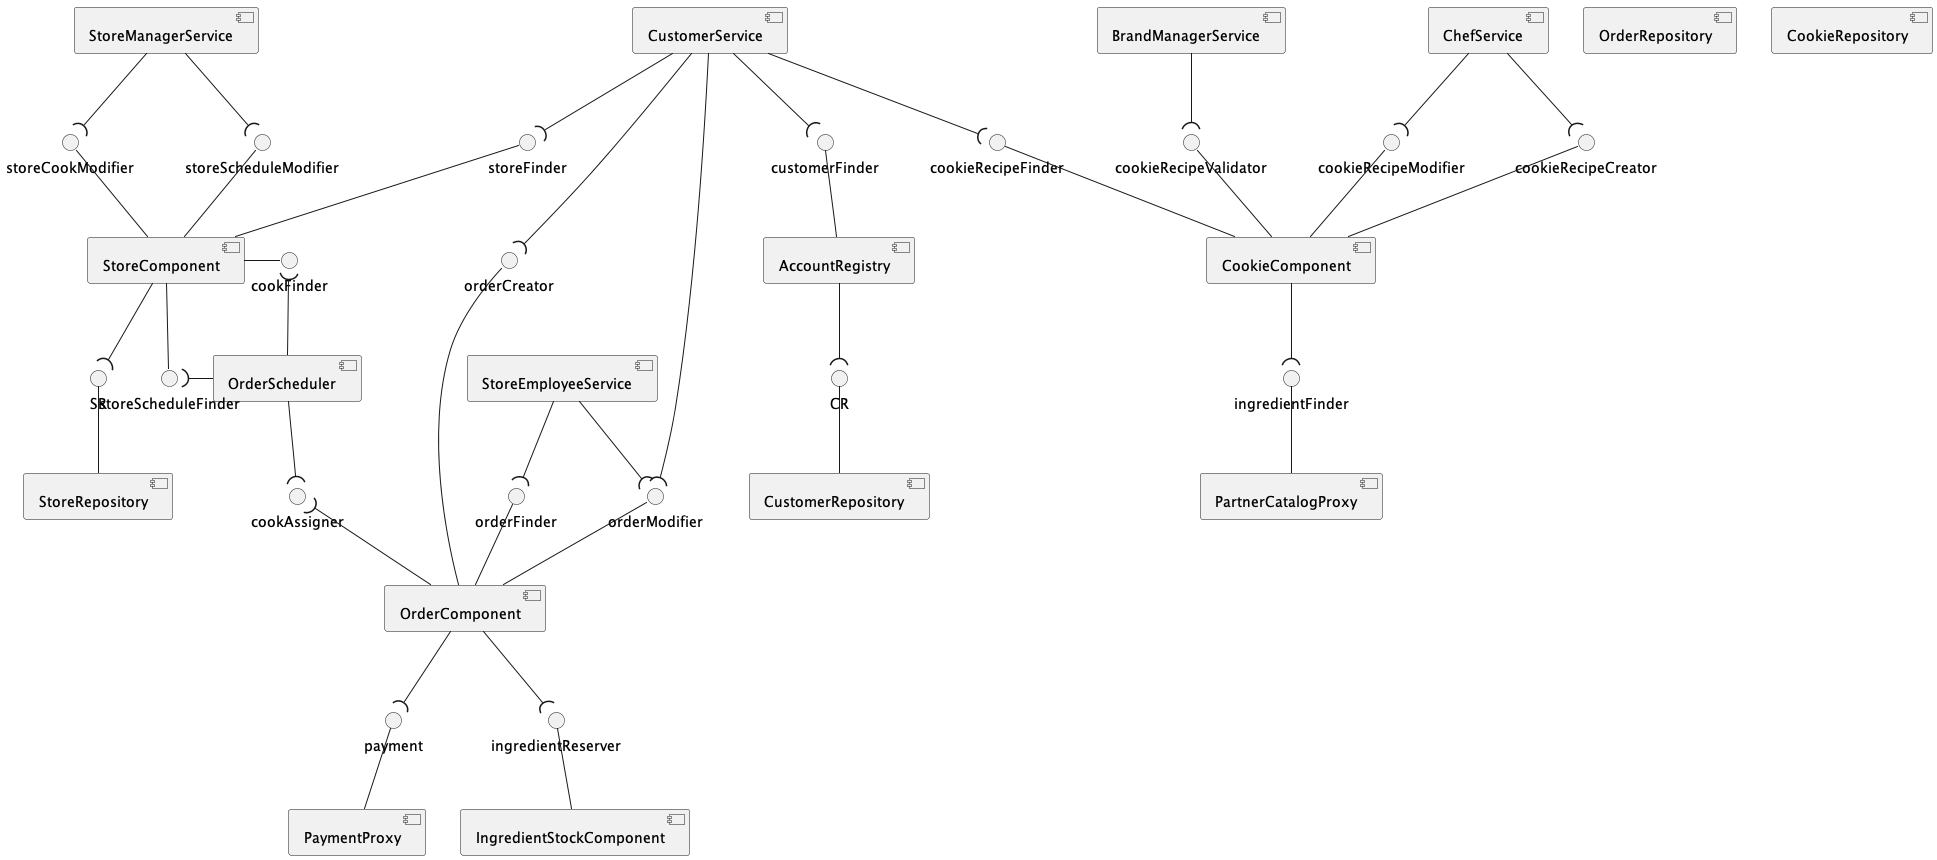
\includegraphics[width=1\textwidth]{component-diagram}
\centering
\caption{Diagramme de Composants Spring}
\label{uml:component}
\end{figure}
\paragraph{Pour migrer} notre code d'une conception OOP vers une approche par composant, nous nous sommes appuyés sur notre 
conception initiale qui comportait déjà une décomposition des classes en fonction des fonctionnalités métier recherchées,
ainsi que les services respectifs chargés d'offrir l'accès à ces fonctionnalités.

\paragraph{}Comme certaines de nos classes de "service" initiales avaient les lignes brouillées entre leurs responsabilités, nous avons opté pour une approche de ségrégation d'interface pour visualiser quelle classe de service prenait en charge quelle responsabilité.

\paragraph{}Sur cette base, les modifications suivantes ont été apportées :
Nous avons séparé notre StoreService (maintenant appelé StoreComponent), en deux composants distincts : StoreComponent et IngredientStockComponent. Comme la classe intiale avait deux grandes responsabilités, la première étant de gérer les préoccupations des magasins et la seconde étant de gérer méticuleusement les stocks d'ingrédients, nous les avons séparés en deux composants. 

\paragraph{}Comme le montre le diagramme des composants, la classe IngredientStockComponent expose deux interfaces : ingredientReserver pour gérer la réservation et la libération des ingrédients en stock, et ingredientModifier pour gérer les quantités réelles en stock au fur et à mesure de l'arrivée de nouveaux lots. 

\paragraph{Le StoreComponent,} il a été restreint au périmètre de la gestion des plannings des magasins (pour leur interrogation et leur modification), et de leurs cuisiniers (pour leur interrogation et la modification de leur planning). 
\paragraph{OrderScheduler} a été définit comme un composant, car il se charge de gérer le planning des cuisiniers et l'affectation des commandes aux cuisiniers respectifs.  Il n'expose donc qu'une seule interface qui est : cookAssigner. 
\paragraph{Le CookieService} initial a été renommé en un CookieComponent qui expose les interfaces nécessaires pour gérer la logique de soumission, d'ajout, de confirmation et d'interrogation des différentes recettes : cookieRecipeFinder, cookieRecipeValidator, cookieRecipeCreator, cookieRecipeModifier.
\paragraph{AccountService} a été renommé AccountRegistry, et a été modifié de manière à ce qu'il implémente deux interfaces : un accountCreator et un customerFinder pour exposer les services derrière la logique d'inscription et de recherche d'informations d'identification.
\paragraph{Les "services"} originaux qui étaient des proxies sont devenus des connecteurs, c'est-à-dire des composants qui fournissent une interface pour des services externes : les API. Par exemple : PaymentProxy, TooGoodToGo, et PartnerCatalogProxy.
\paragraph{OrderComponent,} basé à l'origine sur OrderService, a été conçu de manière à exposer les services de création d'une commande, de sa recherche, de sa modification et de sa confirmation. Les interfaces respectives sont : orderCreator, orderModifier, orderFinder et orderFinalizer. 

\paragraph{}Comme ce composant fait beaucoup de travail de base, il dépend de plusieurs interfaces importantes pour le réaliser, notamment : Payment, cookAssigner, et ingredientReserver pour passer à la caisse.
\paragraph{}Nous n'avons pas mentionné le rôle que jouent les composants "Repository" dans la décomposition ci-dessus, car ces composants sont simplement chargés de gérer l'état de la base de données "en direct", sans logique commerciale apparemment intéressante.
\paragraph{Pour conclure,} toutes nos classes 'Façade' suffixées 'System' auparavant, ont été transformées en services dans l'approche par composant, car ces classes sont devenues responsables de l'exposition des abstractions les plus élevées et des points d'accès directs aux différentes caractéristiques et fonctionnalités du système :
\paragraph{CustomerService:} offre des services d'authentification via Authenticator tels que la connexion et l'inscription, des services liés aux commandes tels que le passage d'une commande et la spécification de ses propriétés (heure et lieu d'enlèvement) et de ce qu'elle concerne : cookies génériques ou cookie de partie personnalisé, etc. via orderPlacer, orderHistoryViewer, tooGoodToGoSubscriber, cookiePersonalizer et notificationReceiver. A utiliser par un client régulier.
\paragraph{BrandManagerService:} expose des fonctionnalités de validation des recettes et de gestion des prix à utiliser par le gestionnaire de la marque par le biais de recipeValidator et cookiePriceManager.
\paragraph{ChefService:} expose des fonctionnalités liées aux recettes qui ont un impact sur le catalogue ; soumission et modification en cas d'acceptation, à utiliser par les chefs de la marque à travers recipeSubmitter et cookieRecipeManger.
\paragraph{StoreManagerService:} expose les fonctionnalités liées au magasin et destinées à être utilisées par le gestionnaire du magasin, à savoir : les taxes et la modification du calendrier du magasin par le biais de scheduleModifier et taxesModifier.
